% !TEX root = ../main.tex
\chapter{General Project Context}
\label{chap:general-project-context}

\section*{Introduction}

This chapter presents the organization that hosted the end-of-study internship. It begins with an overview of Oracle Corporation and its development, then introduces the Morocco Advanced Development Center (MADC) and Oracle Labs. It also describes Oracle's organizational structure and culture before presenting the organization and management of the internship project.


\section{Host Organization}

Businesses, technology companies, and public-sector organizations depend on databases and cloud services to manage their infrastructure, along with core enterprise systems such as ERP, CRM, EPM, and SPM. These technologies are now essential to their daily operations.

Oracle is a leading U.S. multinational technology company specializing in databases, cloud services, and enterprise software. It develops and delivers these technologies to organizations worldwide while placing a strong emphasis on innovation, reliability, and customer satisfaction.

\section{Oracle Corporation}


\begin{figure}[H]
    \centering
    
\includegraphics[width=0.5\textwidth]{Logos/Logo_oracle1.png}
    \caption{Oracle logo}
    \label{fig:oracle-logo}
\end{figure}

\subsection{History}


Oracle Corporation is one of the world's largest enterprise software and cloud-computing companies. Its history began in 1977, when Larry Ellison, Bob Miner, and Ed Oates founded Software Development Laboratories (SDL) in Santa Clara, California. Their objective was to commercialize the emerging concept of the relational database. The company developed one of the first commercial relational database management systems and launched Oracle Version 2 in 1979. It was renamed Oracle Systems Corporation in 1983 and subsequently became a major provider of database technology.

During the 1980s, Oracle experienced rapid growth and went public in 1986. Although the company faced a serious financial crisis in 1990 due to accounting issues, it recovered under Larry Ellison's leadership and expanded beyond databases into enterprise software.

In the 2000s, Oracle expanded through major acquisitions, including PeopleSoft, Siebel Systems, BEA Systems, and Sun Microsystems. These acquisitions brought technologies such as Java and MySQL into Oracle's portfolio. During the 2010s and 2020s, Oracle strengthened its focus on cloud computing through Oracle Cloud Infrastructure (OCI) and cloud-based business applications.

Today, Oracle is one of the world's largest technology companies, providing database systems, cloud infrastructure, enterprise applications, and AI services to organizations worldwide.

\subsection{Oracle MADC}

\begin{figure}[H]
    \centering
    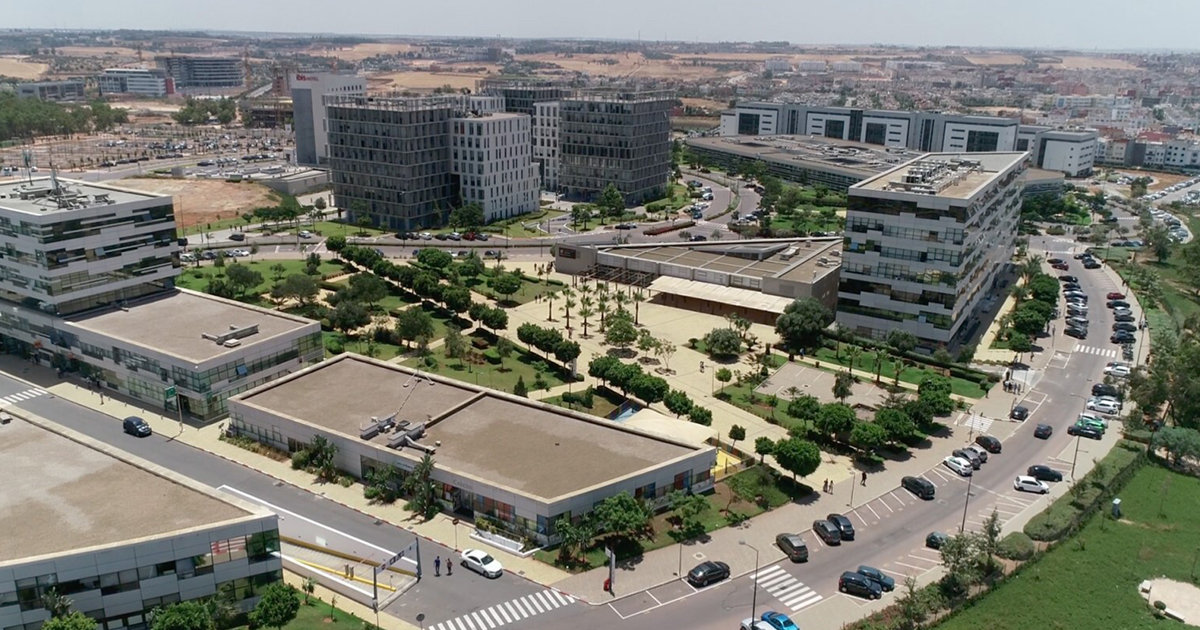
\includegraphics[width=0.5\textwidth]{Figures/Oracle MADC Location.png}
    \caption{Location of Oracle MADC}
    \label{fig:oracle-madc-location}
\end{figure}

The Morocco Advanced Development Center (MADC), established by Oracle Corporation in Casablanca, is Oracle's first R\&D center in Africa. Opened in 2015, it is one of Oracle's principal development centers in the EMEA region. The center brings together software developers, engineers, researchers, and project managers who contribute to projects across several Oracle product lines.

Their work covers fields such as artificial intelligence, augmented, virtual, and mixed reality, big-data analytics, blockchain, cloud computing, cybersecurity, the Internet of Things, machine learning, mobile computing, and serverless computing. MADC also supports graduate recruitment, internship programs, and research collaboration with local academic institutions. Its teams have contributed to Oracle Cloud Infrastructure (OCI), Autonomous Data Warehouse (ADW), and other Oracle products and services.

\begin{figure}[H]
    \centering
    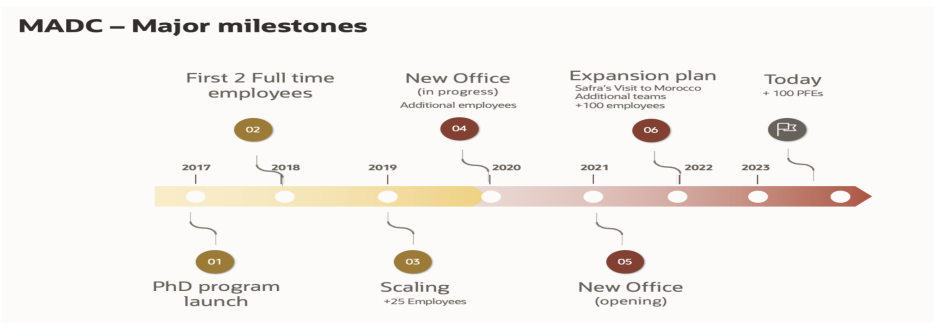
\includegraphics[width=0.99\textwidth]{Figures/MADC Major milestones.png}
    \caption{Major milestones of Oracle MADC}
    \label{fig:madc-major-milestones}
\end{figure}

\subsection{Oracle Labs}
Oracle Labs, the company's research organization, focuses on emerging technologies that may shape future Oracle products and services. Its researchers investigate innovative approaches and undertake projects involving substantial technical uncertainty or long-term research challenges. The objective is to transform research outcomes into practical technologies with measurable industrial impact. For example, work associated with Oracle's research activities has contributed to areas such as the Java programming language and chip multithreading.

Oracle Labs plays a significant role in Oracle's research and development efforts. Its diverse research portfolio helps Oracle identify problems, devise innovative solutions, and develop products that support future growth and innovation.
\begin{figure}[H]
    \centering
    
\includegraphics[width=0.4\textwidth]{Logos/oracle labs logo.png}
    \caption{Oracle Labs logo}
    \label{fig:oracle-labs-logo}
\end{figure}

\subsection{Organizational Structure}
Oracle combines a hierarchical management structure with product-, service-, and region-oriented business units. The Board of Directors oversees the company's strategic direction and performance, while the executive leadership team coordinates its operations. Functional departments such as sales, marketing, finance, human resources, legal affairs, and information technology support the different business units.

Within this matrix structure, employees may collaborate across technical functions, products, and geographical regions. This organization supports coordinated decision-making while enabling multidisciplinary teams to work toward shared objectives.

\subsection{Organizational Culture}
Oracle has a strong corporate culture that prioritizes innovation, customer focus, and excellence. The company's history of innovation, emphasis on customer satisfaction, and commitment to fostering a supportive and collaborative work environment all shape its culture. Oracle's culture emphasizes the following values:

\begin{itemize}
    \item \textbf{Innovation:} The company has a long history of creating products and technologies that have influenced the technology sector. This culture of innovation is supported by investment in research and development and by providing employees with the tools and encouragement needed to test new concepts and create new products.
    \item \textbf{Customer satisfaction:} Oracle's customer-centric approach reflects its commitment to providing products and services that meet its clients' needs. Employees are encouraged to collaborate closely with clients, understand their requirements, and develop suitable solutions.
    \item \textbf{Quality:} Oracle is committed to high-quality operations, products, and services. The company expects its employees to strive for excellence and provides them with the tools, resources, and support required to succeed.
    \item \textbf{Collaboration and teamwork:} Effective collaboration is essential to achieving Oracle's goals and delivering value to customers. The company encourages employees to work across departments and functions and provides tools and resources that facilitate communication and collaboration.
\end{itemize}

Overall, Oracle's organizational culture is characterized by a commitment to innovation, customer focus, excellence, collaboration, and teamwork. These values are reflected in the company's products, services, and operations and guide employees across its different organizational levels.

\subsection{The Data Intelligence Services Team}

The Data Intelligence Services (DIS) team is an engineering group within
Oracle that delivers reusable data analytics and machine-learning capabilities
for SaaS applications running on Oracle Cloud Infrastructure. By providing a
standardized platform, DIS allows product teams to focus on industry-specific
business use cases without independently building and operating the underlying
analytics infrastructure. This approach encourages consistency, efficiency,
and reuse across Oracle's Global Business Units.

The team designs, develops, and maintains the platform components that support
data ingestion, storage, processing, visualization, and machine-learning
workloads. These components integrate with cloud services such as Autonomous
Database, Oracle Analytics Cloud, Object Storage, and other OCI data and AI
services. The team also applies Oracle's security, architectural, and
cloud-native engineering practices and collaborates with service owners and GBU
partners to analyze requirements, deliver platform capabilities, and resolve
integration issues.

The internship is conducted within the DIS team, with a principal focus on the
visualization domain and the lifecycle of Oracle Analytics Server and Oracle
Analytics Cloud environments. The activities include analyzing onboarding and
migration workflows, validating analytics artifacts, investigating integration
issues, and contributing to OAC cross-region disaster-recovery automation. The
work is carried out under the guidance of Ajay Kumar as technical mentor and
Sunil Padiyar as dotted-line manager, in collaboration with engineers and
architects from the services involved in these workflows.

Figure~\ref{fig:internship-organizational-chart} presents a simplified view of
the internship's organizational and technical supervision.

\begin{figure}[H]
    \centering
    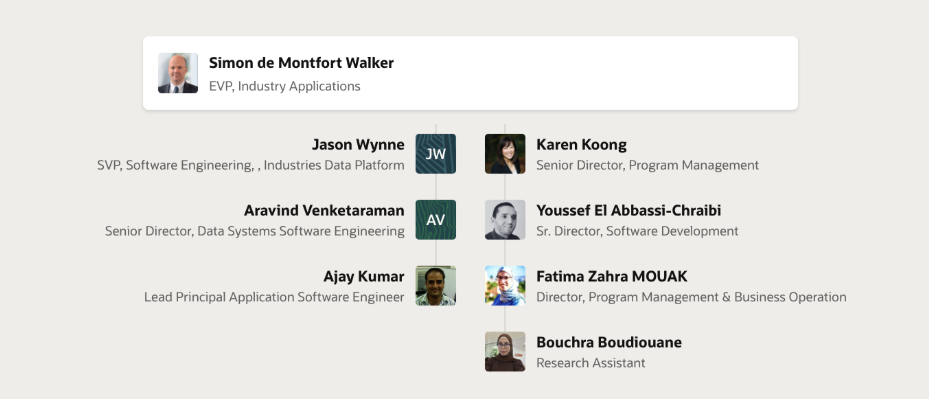
\includegraphics[width=0.9\textwidth]
    {Figures/internship-organizational-chart.png}
    \caption{Simplified organizational chart of the internship within DIS}
    \label{fig:internship-organizational-chart}
\end{figure}

\section{Project Management}

The internship was carried out within an existing engineering team whose
activities include platform development, cloud operations, integration, and
quality assurance. The work was therefore organized as part of the team's
regular delivery process rather than as an isolated academic project. This
organization provided access to real requirements, collaborative technical
reviews, and non-production environments used to validate the developed
features.

\subsection{Onboarding and Integration}

The integration period established the organizational and technical context
required to contribute to the project. It began with an introduction to the
team, its responsibilities, and the principal services of the Data
Intelligence Services platform. Knowledge-transfer sessions and internal
documentation were then used to become familiar with Oracle Analytics Server,
Oracle Analytics Cloud, tenant onboarding, and the platform's development and
deployment processes.

The technical integration progressed incrementally. The first activities
focused on understanding existing workflows and executing guided operations in
development environments. They were followed by analysis and validation
stories, and then by implementation tasks involving source-code changes,
automated tests, code review, continuous integration, and deployment
verification. This gradual approach reduced the risk associated with modifying
a distributed cloud platform and made it possible to acquire the required
technical autonomy progressively.

\subsection{Project Management Methodology}

\subsubsection{Adopted Methodology: Scrumban}

The DIS team adopts \textbf{Scrumban}, a hybrid Agile methodology combining
Scrum's planning cadence with Kanban's visual workflow management. Work is
organized in two-week sprints, while the task board remains flexible enough to
accommodate feature development, investigation, bug resolution, and
environment-dependent validation activities.

The team holds a daily stand-up meeting of approximately thirty minutes. Each
member reports the work completed since the previous meeting, the work planned
for the day, and any blocking issue. Sprint-planning sessions are held every two
weeks to review the backlog, assess dependencies, and select the stories to be
addressed during the next iteration. Progress and work logs are maintained in
Jira so that the current state of each activity remains visible.

This methodology is appropriate for the project because the implementation
depends on several microservices, cloud services, and service owners. A task may
be interrupted by an unavailable environment, an unresolved product limitation,
or a change required in another repository. Scrumban preserves a regular
planning rhythm while allowing priorities to be adjusted when these constraints
appear.

Figure~\ref{fig:dis-scrumban-board} will present the Scrumban board used to
visualize and monitor the team's work. Before including the final screenshot,
confidential issue details and personal information must be removed or masked.

\begin{figure}[H]
    \centering
    \IfFileExists{Figures/dis_team_scrumban_board.png}{%
        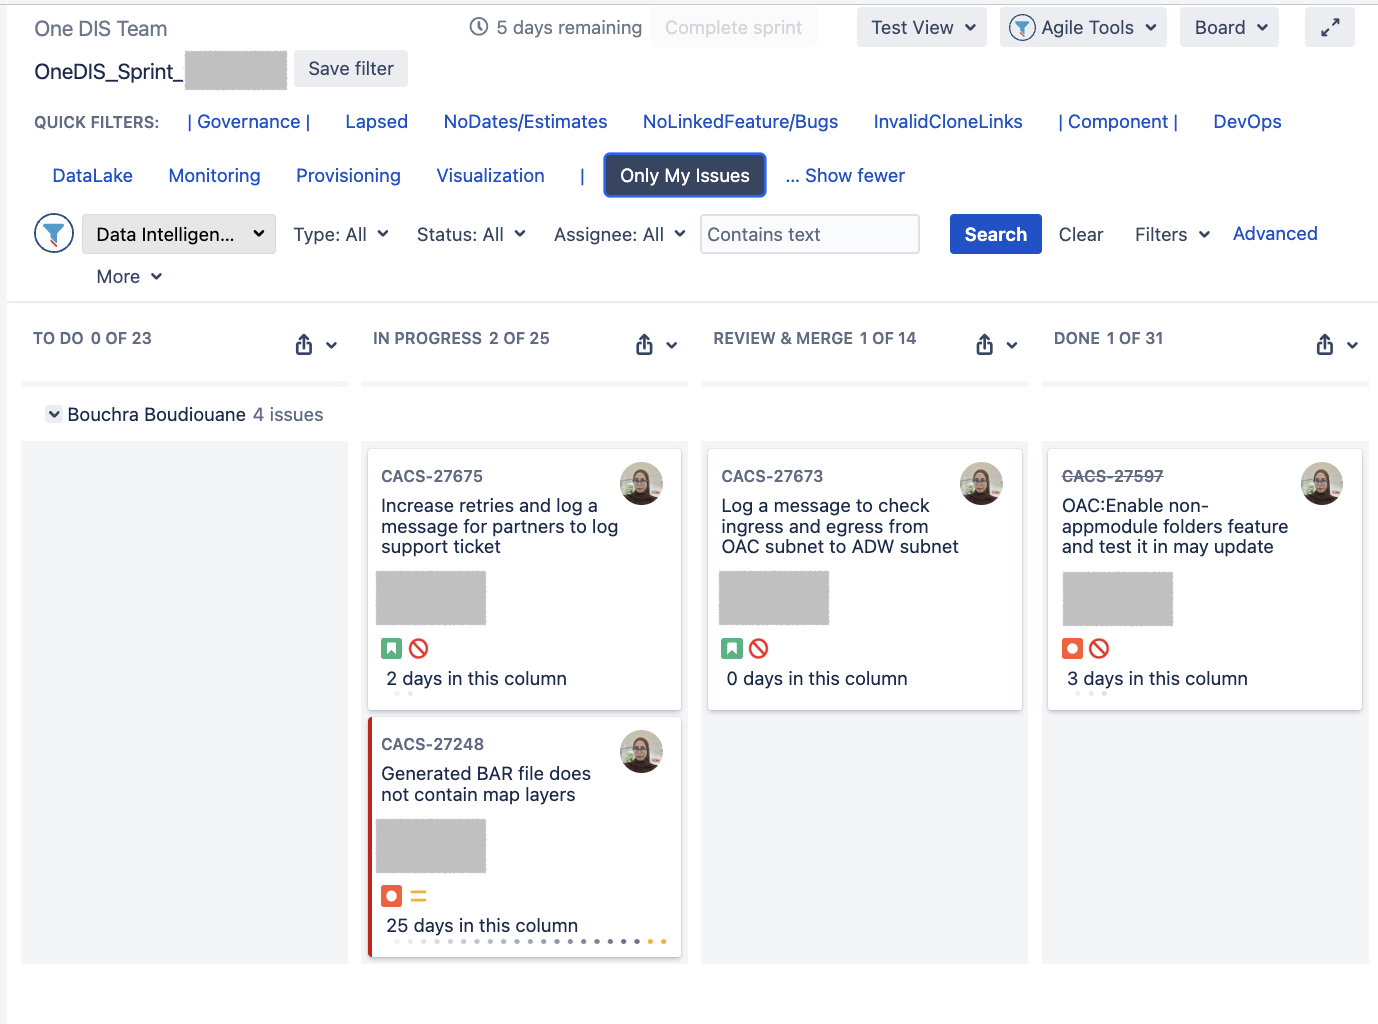
\includegraphics[width=0.95\textwidth]
        {Figures/dis_team_scrumban_board.png}%
    }{%
        \fbox{\parbox[c][6cm][c]{0.9\textwidth}{\centering
        Reserved space for a sanitized screenshot of the DIS Team Scrumban Board.}}%
    }
    \caption{DIS Team Scrumban Board}
    \label{fig:dis-scrumban-board}
\end{figure}

\subsubsection{Agile and Kanban Principles}

Agile development promotes incremental delivery, frequent feedback, and
adaptation to changing requirements. Instead of treating the complete solution
as one delivery, the DR feature is divided into stories covering request
validation, workflow execution, backup restoration, status reporting, retry,
rollback, and cleanup. Each increment can therefore be reviewed and validated
before the complete feature is tested end to end.

Kanban complements this iterative organization by visualizing the flow of work.
A story is moved across the board according to its current state, such as
\textit{To Do}, \textit{In Progress}, \textit{Review and Merge}, and
\textit{Done}. The board also exposes work that is blocked or placed on hold,
which helps the team identify dependencies and avoid losing visibility over
unfinished activities.

\subsubsection{Application within the Internship}

For each assigned story, the working cycle consists of analyzing the requirement,
studying the existing implementation, identifying the affected services,
developing or validating the proposed change, adding automated tests, and
submitting the result for peer review. After the continuous-integration pipeline
succeeds, the corresponding container image can be deployed in a non-production
environment for integration or end-to-end validation. Technical findings, test
evidence, and work logs are recorded on the story to maintain traceability.

\subsection{Internship Planning}

The internship was organized into progressive and partially overlapping
phases. Since the work is integrated into the team's evolving backlog, the
planning remains adaptable to new OAC features and external dependencies.
Table~\ref{tab:internship-planning} presents the principal phases and their
expected outputs.

\begin{table}[H]
\centering
\caption{Main phases of the internship}
\label{tab:internship-planning}
\begin{tabularx}{\textwidth}{@{}p{1.5cm}p{3.8cm}X@{}}
\toprule
\textbf{Phase} & \textbf{Focus} & \textbf{Principal outputs} \\
\midrule
1 & Integration and knowledge acquisition & Understanding of DIS, OAS, OAC, tenant onboarding, development practices, and operational tools. \\
2 & Functional analysis and validation & Analysis of migration and visualization workflows, execution of proofs of concept, and identification of integration issues. \\
3 & OAC feature development & Design and implementation of cross-region disaster-recovery capabilities, including recovery status, retry, rollback, restoration, and cleanup behavior. \\
4 & Integration and quality assurance & Unit tests, code review, continuous-integration builds, deployment verification, and end-to-end validation in non-production environments. \\
5 & Documentation and consolidation & Academic report preparation, synthesis of results, documentation of limitations, and integration of additional OAC features addressed later in the internship. \\
\bottomrule
\end{tabularx}
\end{table}

\section{Collaboration Tools}

The internship relied on several complementary tools for communication,
planning, technical documentation, source-code collaboration, and continuous
integration. The following subsections describe their role in the project.

\subsection{Team Communication}

\subsubsection{Slack}

Slack was the principal instant-messaging tool used by the team. Public and
private channels supported daily coordination, technical discussions,
announcements, and communication between the owners of different services. It
was particularly useful for quickly clarifying requirements and dependencies
that involved more than one repository or engineering group.

\begin{figure}[H]
    \centering
    \IfFileExists{Figures/slack.png}{%
        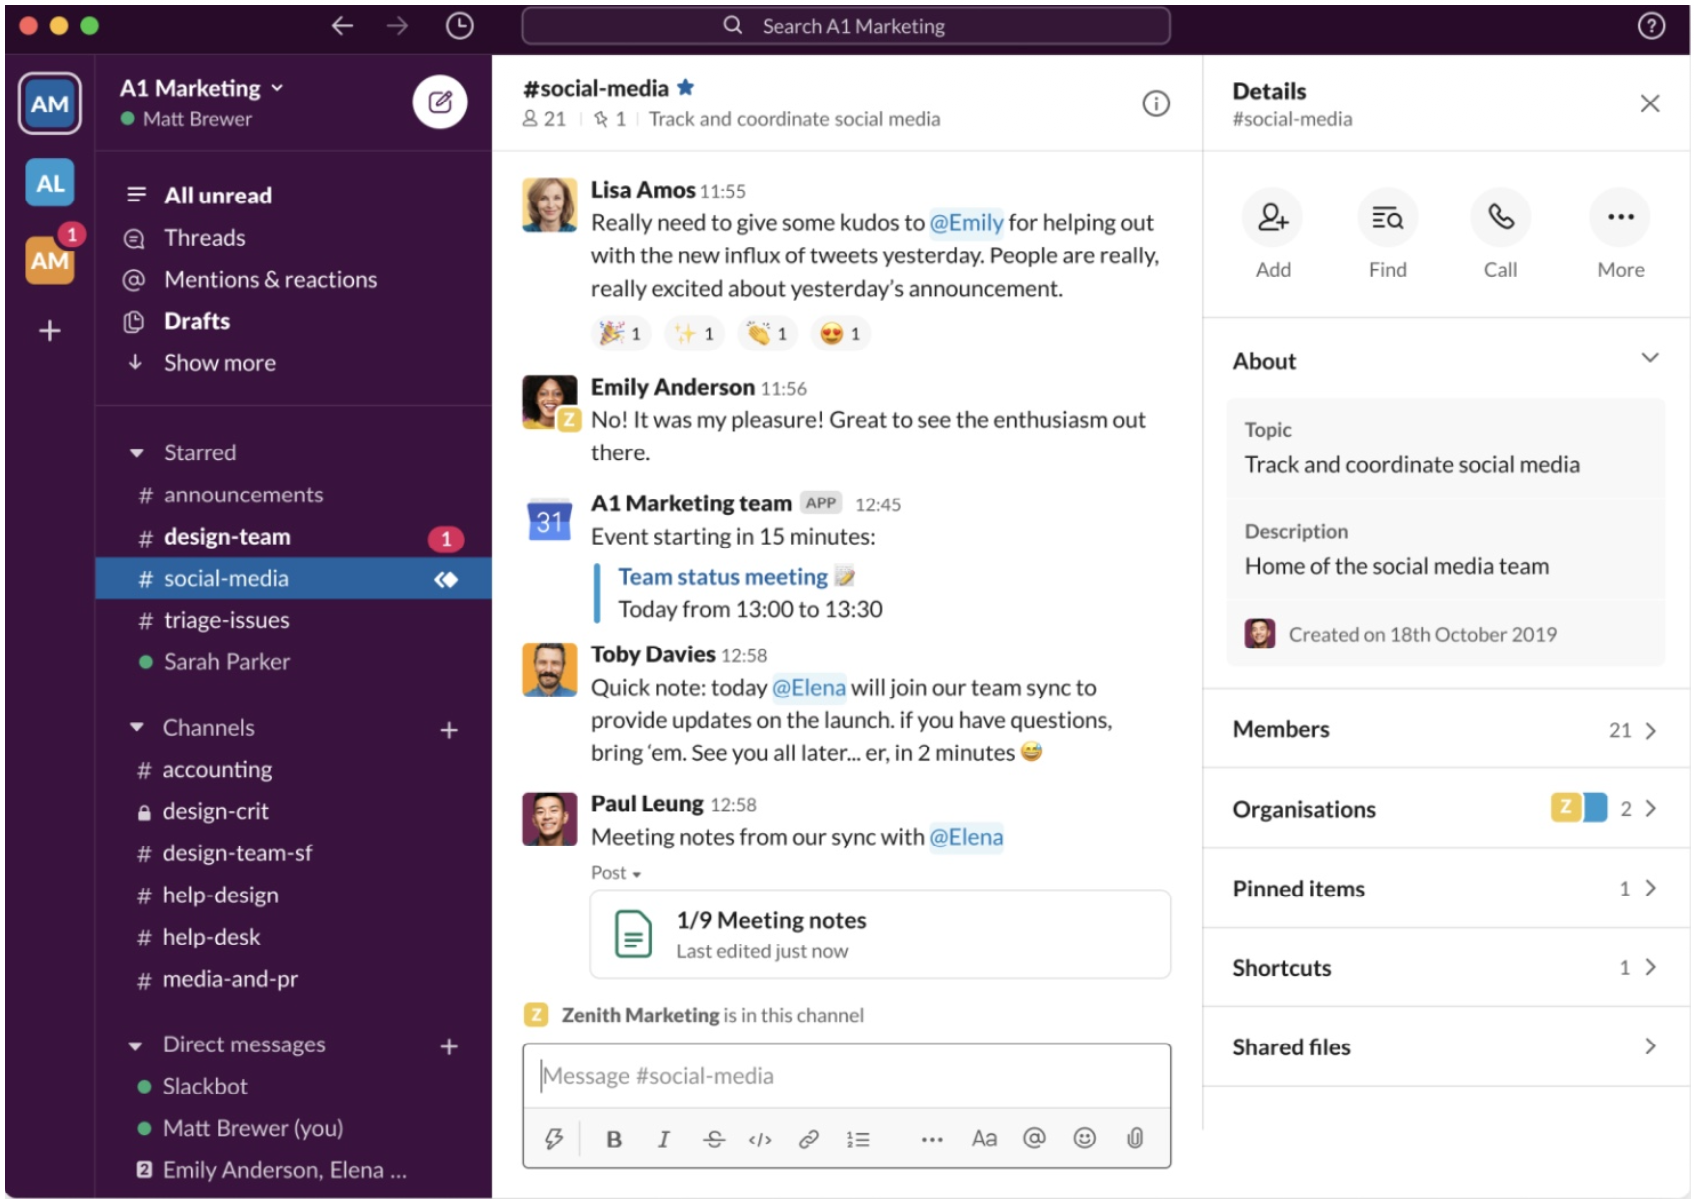
\includegraphics[width=0.82\textwidth]{Figures/slack.png}%
    }{%
        \fbox{\parbox[c][5cm][c]{0.86\textwidth}{\centering
        Reserved space for a sanitized Slack screenshot.}}%
    }
    \caption{Example of team communication through Slack}
    \label{fig:slack-collaboration}
\end{figure}

\subsubsection{Outlook}

Outlook provided email and calendar services for formal communication and
meeting organization. Calendar invitations were used to coordinate daily
meetings, sprint sessions, knowledge-transfer meetings, and technical reviews
with participants from different teams.

\begin{figure}[H]
    \centering
    \IfFileExists{Figures/outlook_calendar.png}{%
        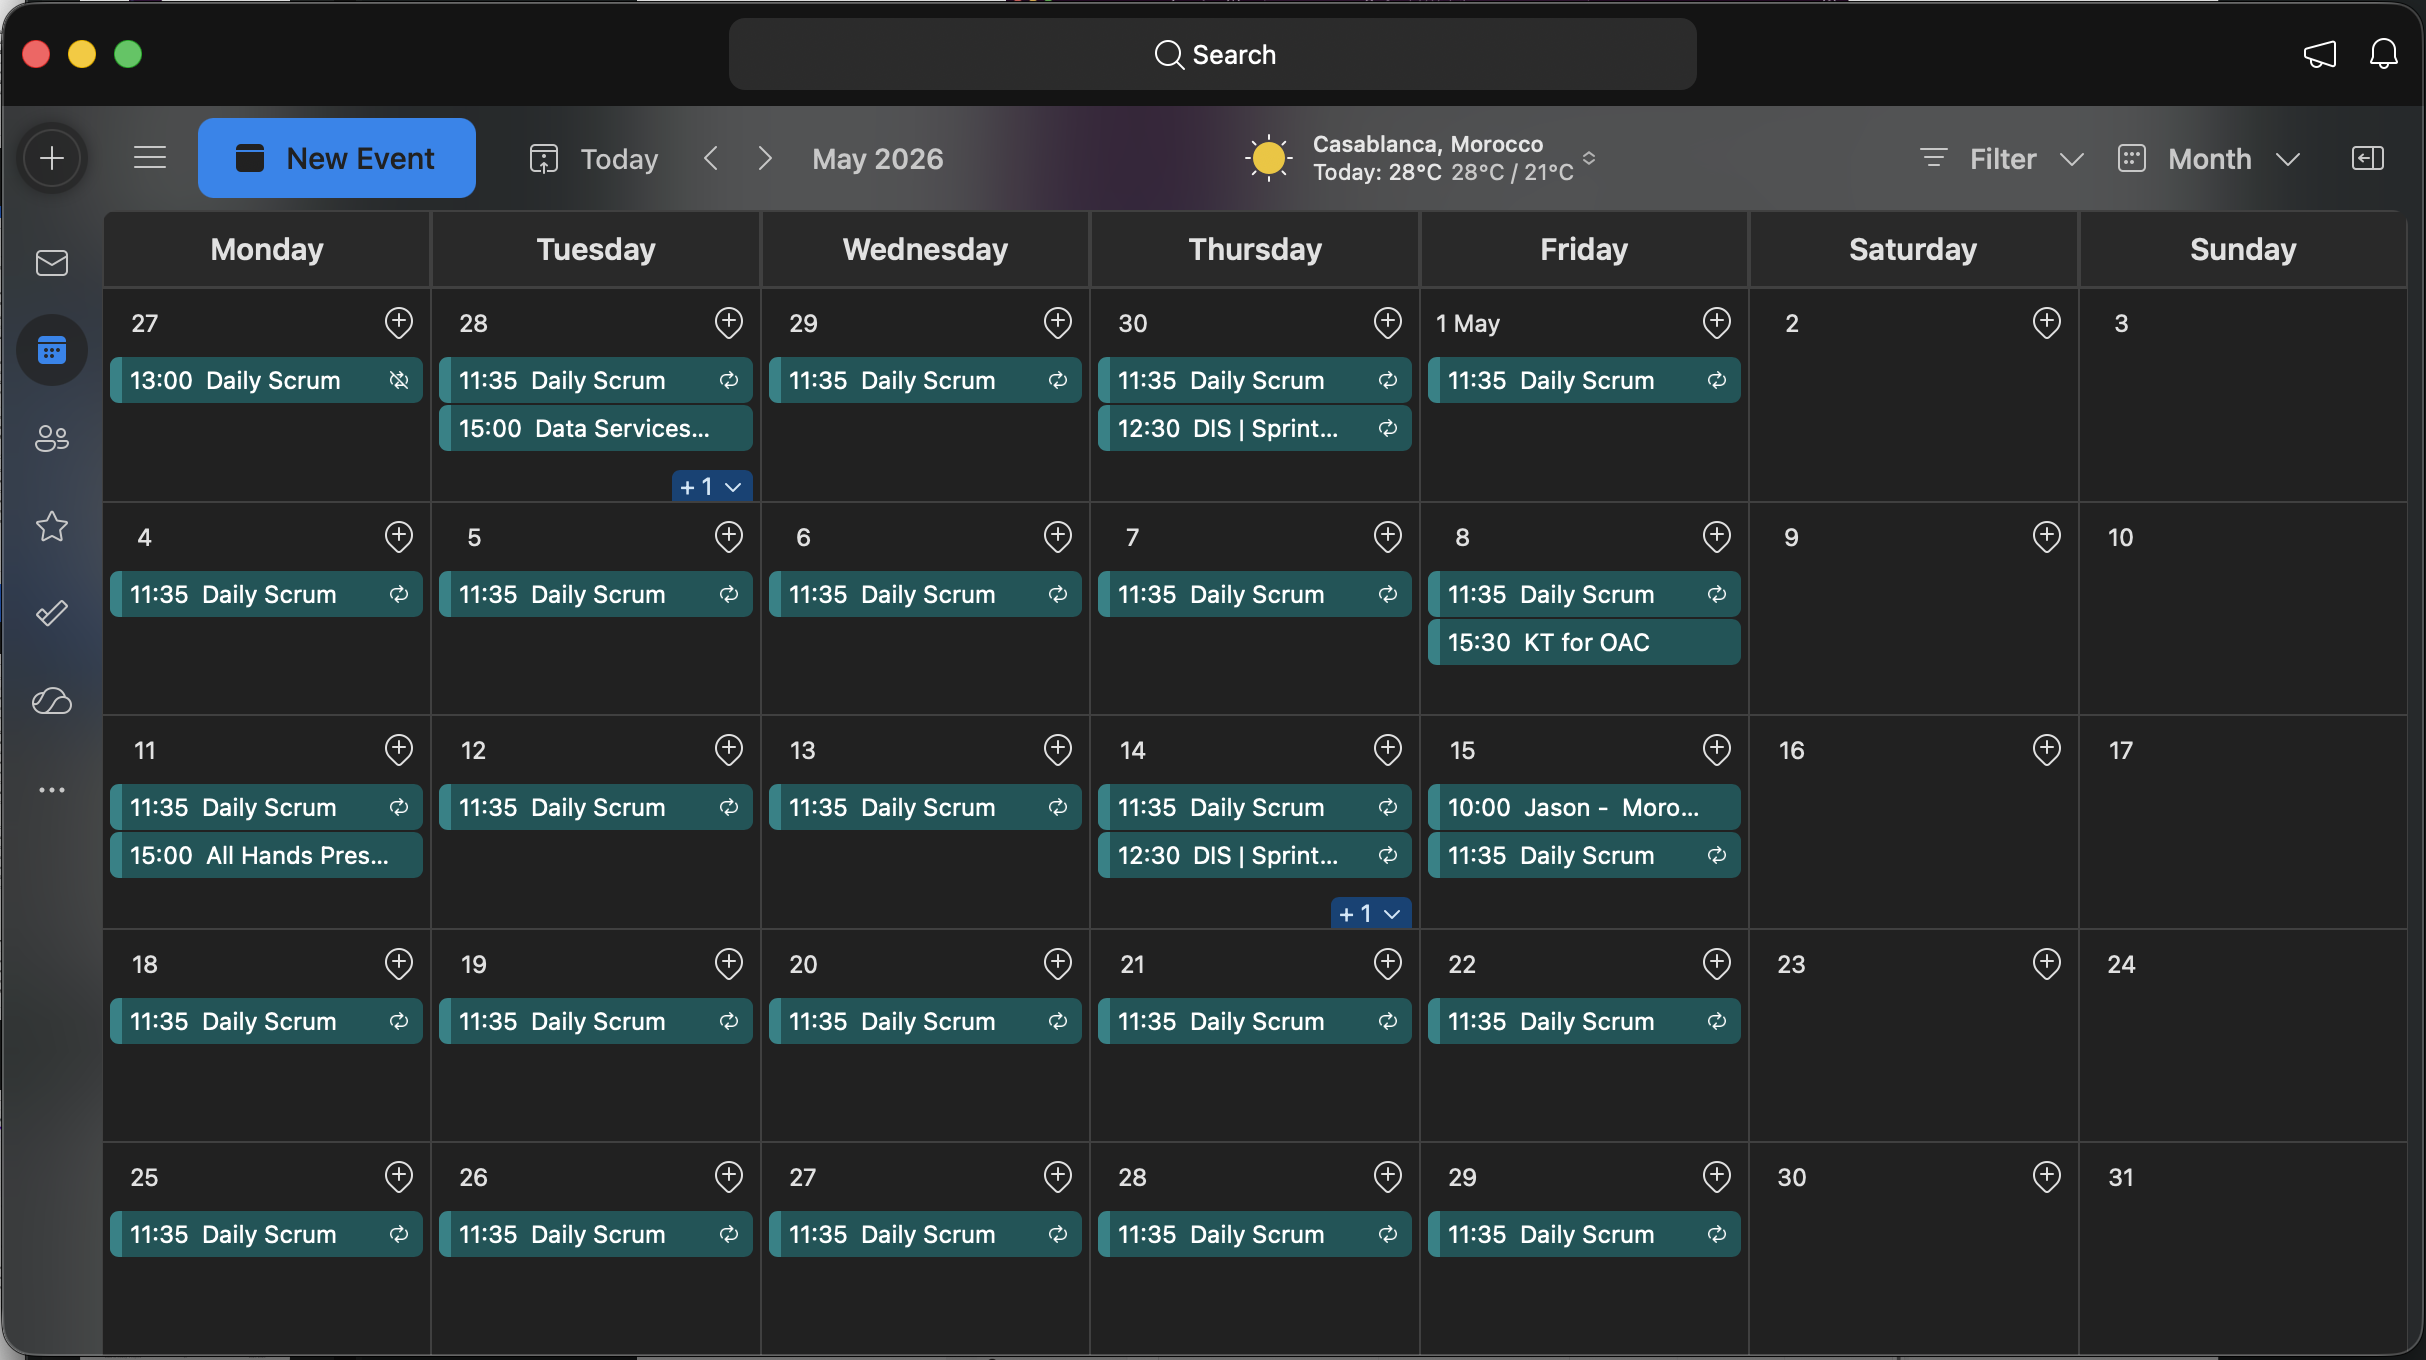
\includegraphics[width=0.82\textwidth]
        {Figures/outlook_calendar.png}%
    }{%
        \fbox{\parbox[c][5cm][c]{0.86\textwidth}{\centering
        Reserved space for a sanitized Outlook calendar screenshot.}}%
    }
    \caption{Meeting organization using Outlook Calendar}
    \label{fig:outlook-calendar}
\end{figure}

\subsubsection{Zoom}

Zoom supported remote meetings and screen sharing. It was used for team
meetings, technical demonstrations, knowledge-transfer sessions, and other
collaborative discussions requiring direct interaction between participants.

\begin{figure}[H]
    \centering
    \IfFileExists{Figures/zoom.png}{%
        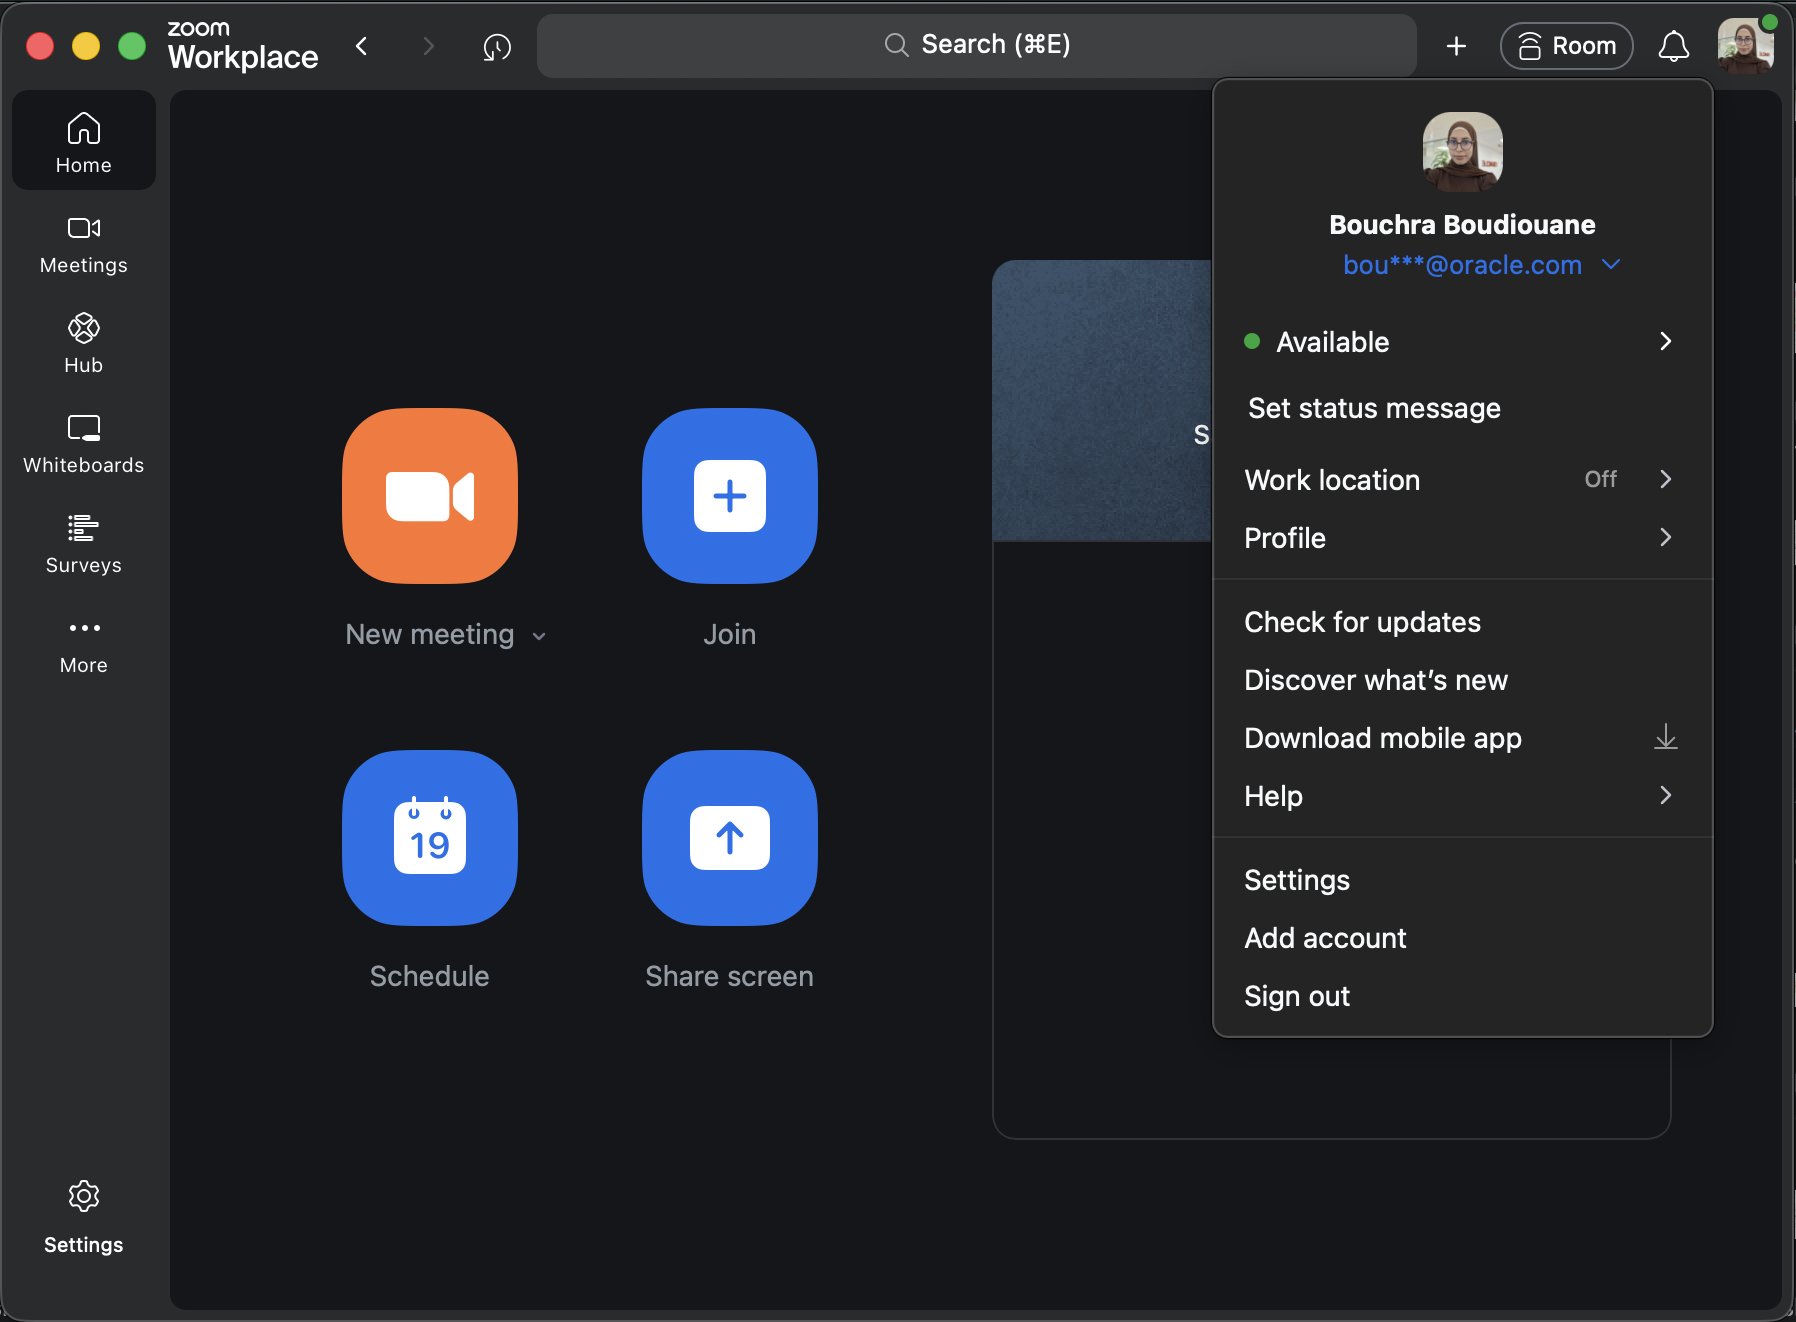
\includegraphics[width=0.78\textwidth]{Figures/zoom.png}%
    }{%
        \fbox{\parbox[c][5cm][c]{0.86\textwidth}{\centering
        Reserved space for a sanitized Zoom meeting screenshot.}}%
    }
    \caption{Remote collaboration through Zoom}
    \label{fig:zoom-collaboration}
\end{figure}

\subsection{Project and Task Management}

\subsubsection{Jira}

Jira was used to manage epics, stories, defects, priorities, dependencies, and
sprint status. Each story provided a traceable location for the requirement,
technical discussion, implementation status, test evidence, and work log. The
workflow states made it possible to distinguish planned work, active
development, code review, completed work, and activities placed on hold.

\begin{figure}[H]
    \centering
    \IfFileExists{Figures/jira_ticket_example.png}{%
        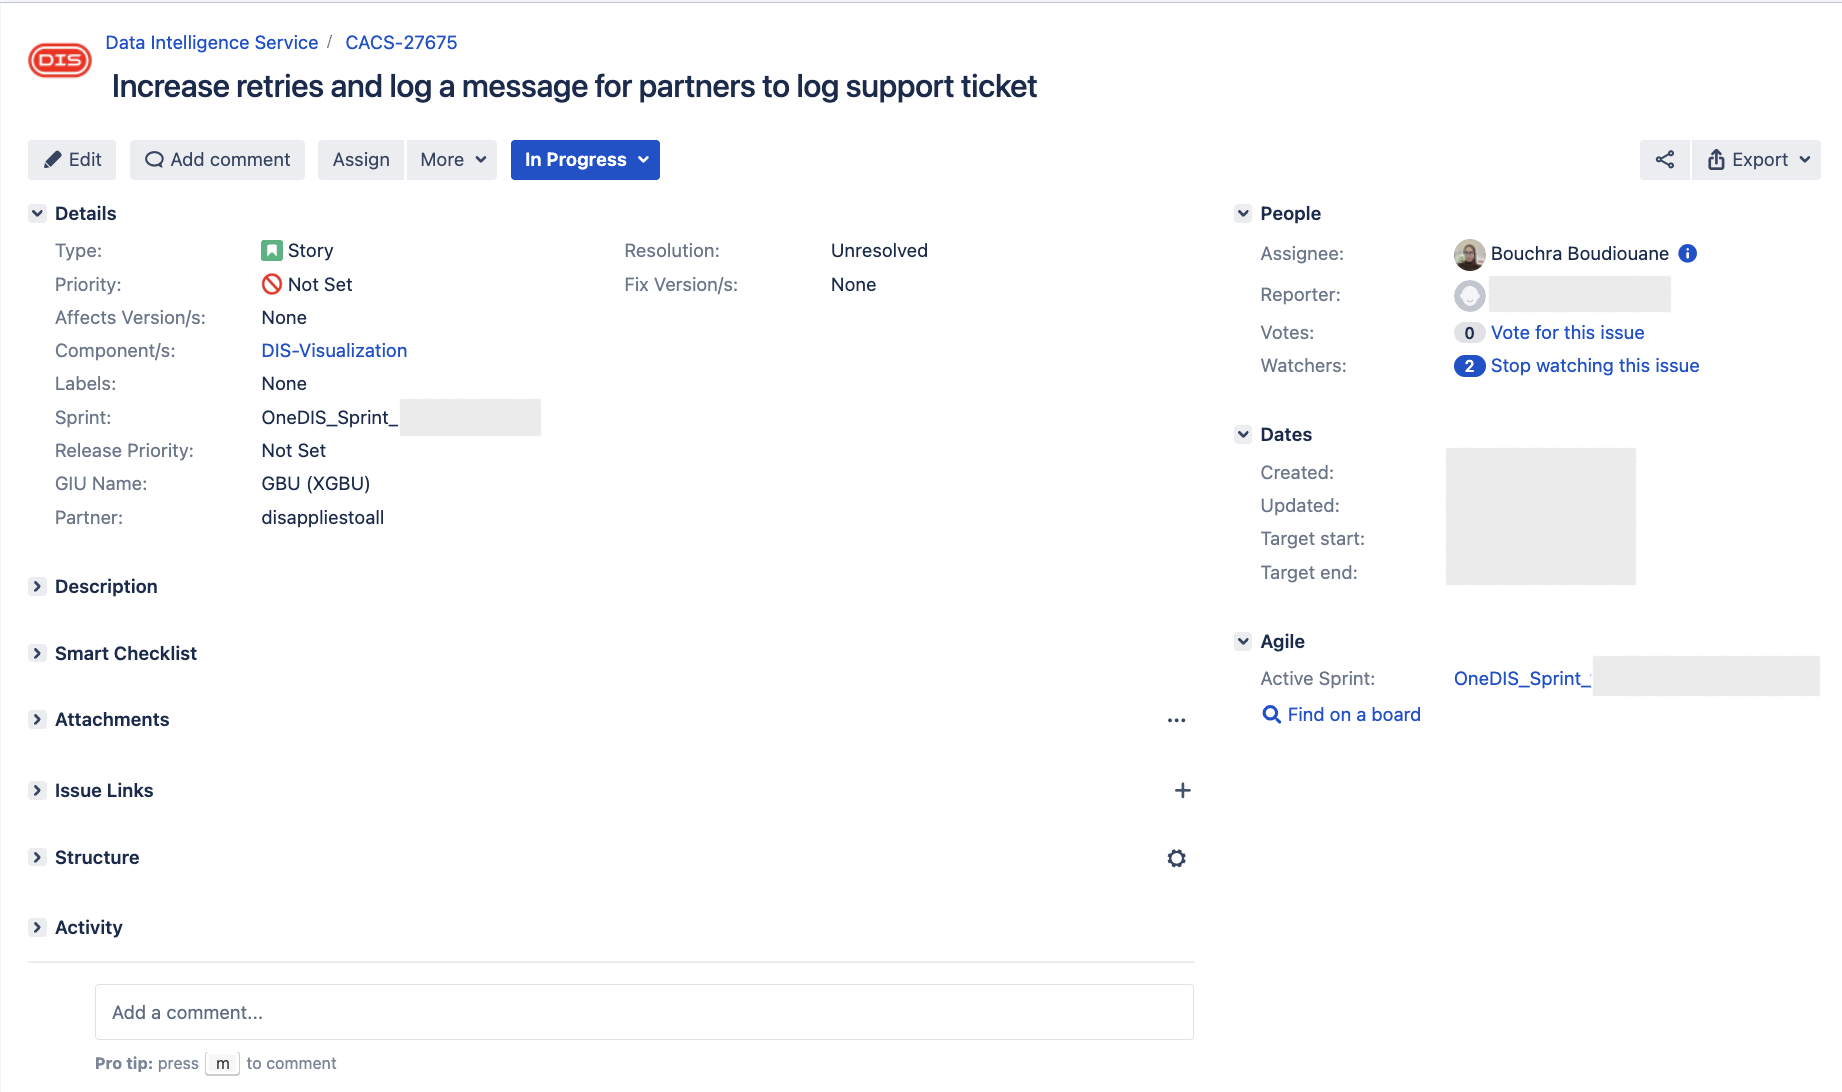
\includegraphics[width=0.9\textwidth]
        {Figures/jira_ticket_example.png}%
    }{%
        \fbox{\parbox[c][5.5cm][c]{0.9\textwidth}{\centering
        Reserved space for a sanitized Jira story example.}}%
    }
    \caption{Example of a project story managed in Jira}
    \label{fig:jira-story-example}
\end{figure}

\begin{figure}[H]
    \centering
    \IfFileExists{Figures/jira_workflow.png}{%
        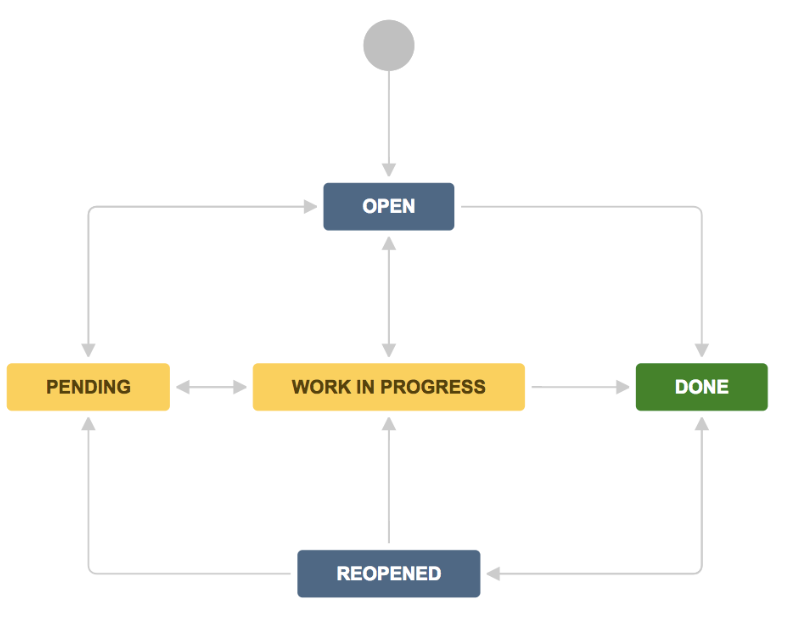
\includegraphics[width=0.9\textwidth]
        {Figures/jira_workflow.png}%
    }{%
        \fbox{\parbox[c][5cm][c]{0.9\textwidth}{\centering
        Reserved space for the Jira story workflow.}}%
    }
    \caption{Principal states of the Jira story workflow}
    \label{fig:jira-story-workflow}
\end{figure}

\subsection{Documentation}

\subsubsection{Confluence}

Confluence served as the team's shared documentation platform. It contained
architecture descriptions, feature requirements, implementation designs,
operational procedures, meeting notes, and knowledge-transfer material. These
documents supported the analysis of existing behavior and provided a common
reference during implementation and review.

\begin{figure}[H]
    \centering
    \IfFileExists{Figures/confluence_design_document.png}{%
        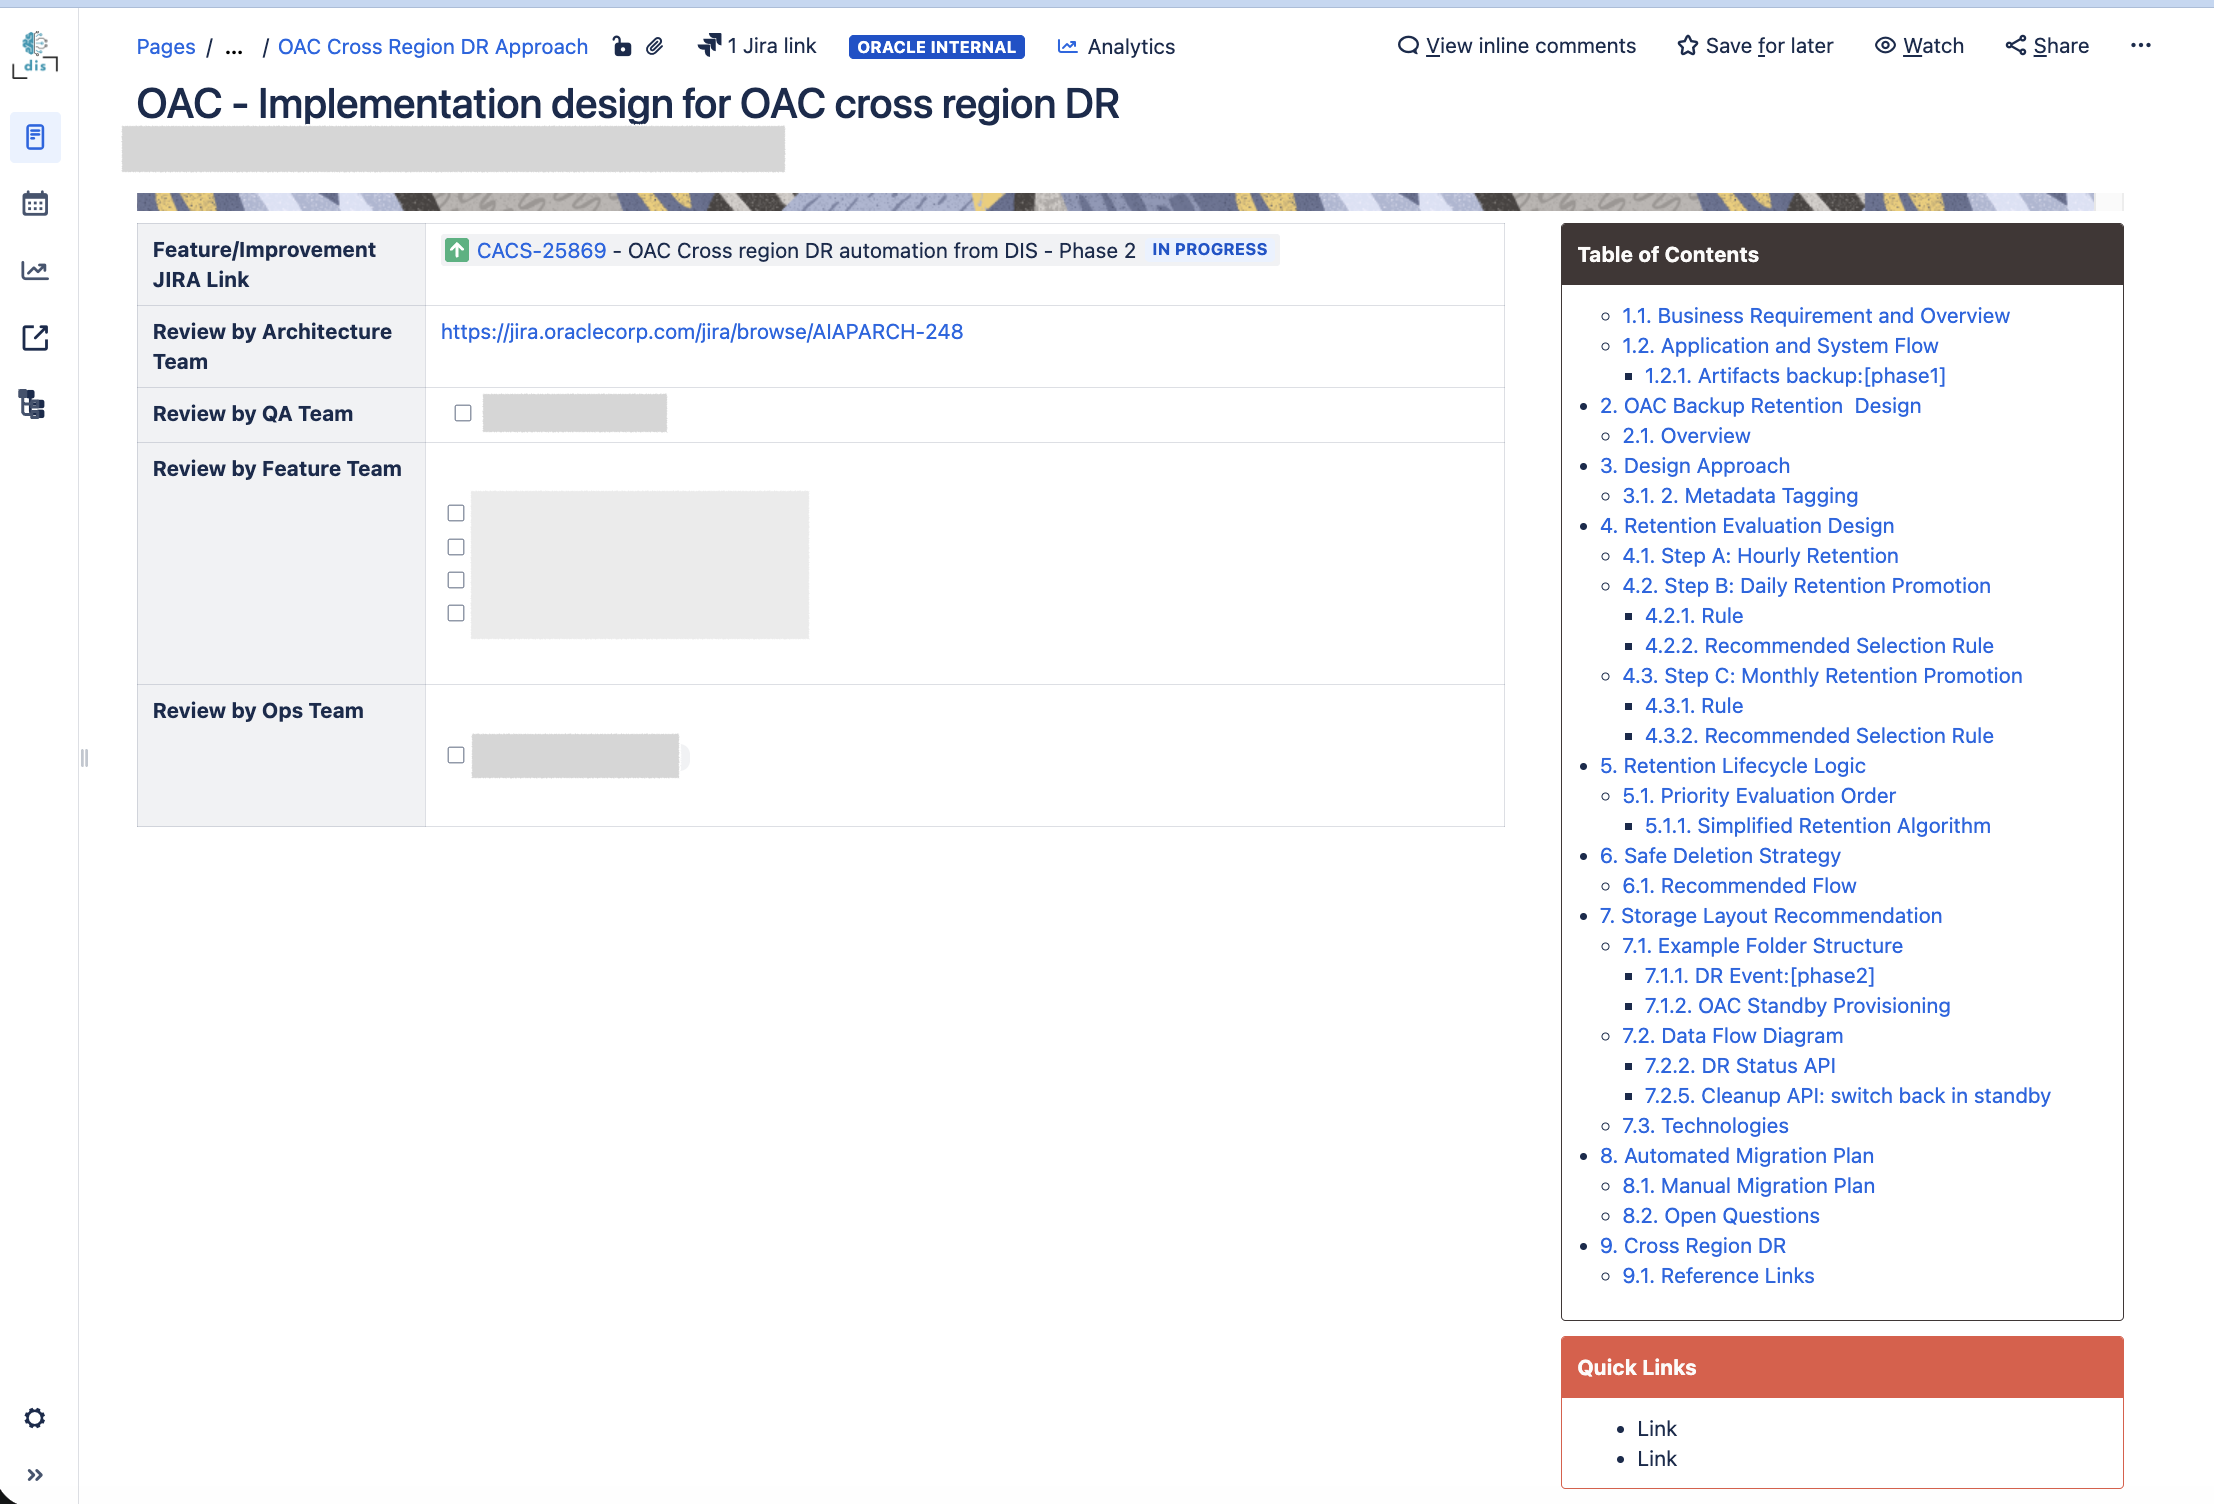
\includegraphics[width=0.9\textwidth]
        {Figures/confluence_design_document.png}%
    }{%
        \fbox{\parbox[c][5.5cm][c]{0.9\textwidth}{\centering
        Reserved space for a sanitized Confluence design document.}}%
    }
    \caption{Example of technical documentation maintained in Confluence}
    \label{fig:confluence-documentation}
\end{figure}

\subsection{Development Collaboration and Delivery}

GitLab was used for source-code management through feature branches, merge
requests, peer review, and change history. Jenkins complemented this process by
executing continuous-integration pipelines, building application packages and
container images, and supporting deployment verification. Together, these
tools connected the implementation and review process to repeatable delivery in
the development environments.

\section*{Conclusion}

This chapter introduced Oracle Corporation and the environment in which the internship was conducted. It highlighted the role of Oracle MADC as a development and research center, the contribution of Oracle Labs to technological innovation, and the organizational principles that support collaboration across the company. It also presented the Agile organization, tools, and progressive planning used to manage the internship activities. This context provides the foundation for understanding the DIS platform and the technical environment presented in the next chapter.
